%---------------------------------------------------------------
\chapter{\LaTeX Examples}

\begin{chapterabstract}
\end{chapterabstract}

\section{}

%-------------------------------------------------------------------------------
\begin{figure}
	\centering
	%\includegraphics[scale=0.4]{pic/index}
	\resizebox{\textwidth}{!}{
		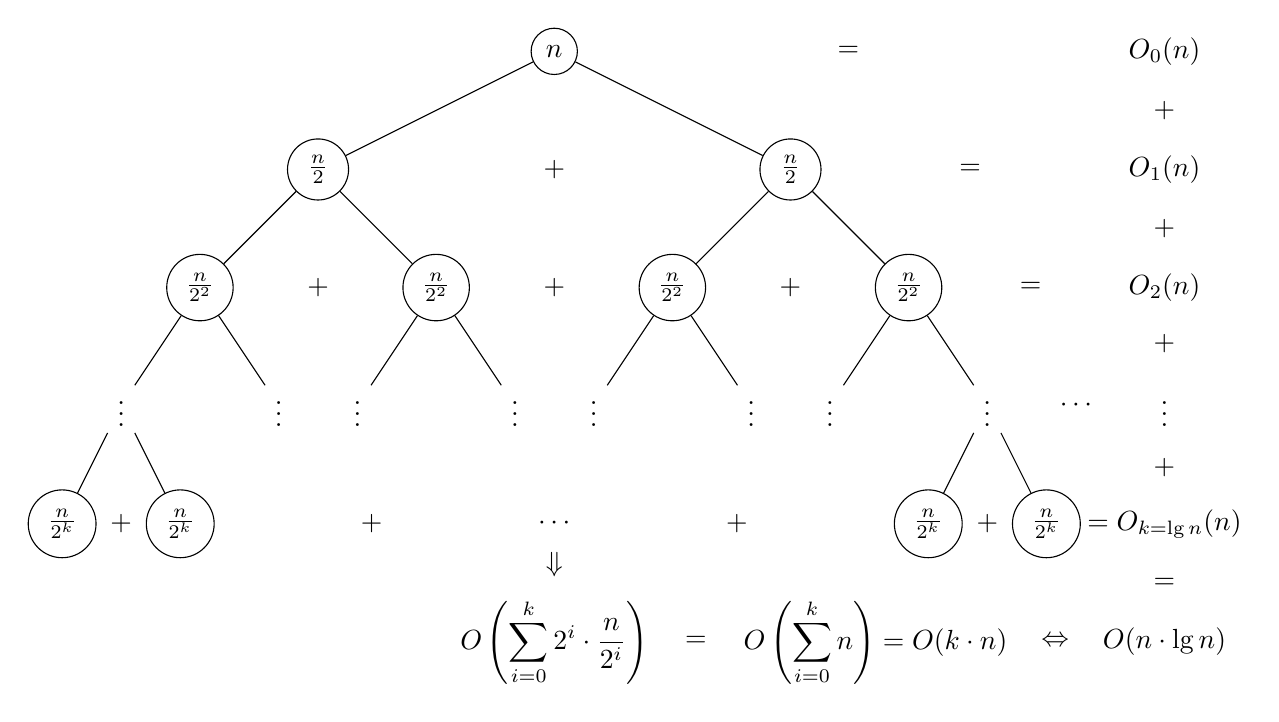
\begin{tikzpicture}[level/.style={sibling distance=60mm/#1}]
			\node [circle,draw] (z){$n$}
			child {node [circle,draw] (a) {$\frac{n}{2}$}
					child {node [circle,draw] (b) {$\frac{n}{2^2}$}
							child {node {$\vdots$}
									child {node [circle,draw] (d) {$\frac{n}{2^k}$}}
									child {node [circle,draw] (e) {$\frac{n}{2^k}$}}
								}
							child {node {$\vdots$}}
						}
					child {node [circle,draw] (g) {$\frac{n}{2^2}$}
							child {node {$\vdots$}}
							child {node {$\vdots$}}
						}
				}
			child {node [circle,draw] (j) {$\frac{n}{2}$}
					child {node [circle,draw] (k) {$\frac{n}{2^2}$}
							child {node {$\vdots$}}
							child {node {$\vdots$}}
						}
					child {node [circle,draw] (l) {$\frac{n}{2^2}$}
							child {node {$\vdots$}}
							child {node (c){$\vdots$}
									child {node [circle,draw] (o) {$\frac{n}{2^k}$}}
									child {node [circle,draw] (p) {$\frac{n}{2^k}$}
											child [grow=right] {node (q) {$ = O_{k = \lg n}(n)$} edge from parent[draw=none]
													child [grow=up] {node (r) {$\vdots$} edge from parent[draw=none]
															child [grow=up] {node (s) {$O_2(n)$} edge from parent[draw=none]
																	child [grow=up] {node (t) {$O_1(n)$} edge from parent[draw=none]
																			child [grow=up] {node (u) {$O_0(n)$} edge from parent[draw=none]}
																		}
																}
														}
													child [grow=down] {node (v) {$O(n \cdot \lg n)$}edge from parent[draw=none]}
												}
										}
								}
						}
				};
			\path (a) -- (j) node [midway] {+};
			\path (b) -- (g) node [midway] {+};
			\path (k) -- (l) node [midway] {+};
			\path (k) -- (g) node [midway] {+};
			\path (d) -- (e) node [midway] {+};
			\path (o) -- (p) node [midway] {+};
			\path (o) -- (e) node (x) [midway] {$\cdots$}
			child [grow=down] {
					node (y) {$O\left(\displaystyle\sum_{i = 0}^k 2^i \cdot \frac{n}{2^i}\right)$}
					edge from parent[draw=none]
				};
			\path (q) -- (r) node [midway] {+};
			\path (s) -- (r) node [midway] {+};
			\path (s) -- (t) node [midway] {+};
			\path (s) -- (l) node [midway] {=};
			\path (t) -- (u) node [midway] {+};
			\path (z) -- (u) node [midway] {=};
			\path (j) -- (t) node [midway] {=};
			\path (y) -- (x) node [midway] {$\Downarrow$};
			\path (v) -- (y)
			node (w) [midway] {$O\left(\displaystyle\sum_{i = 0}^k n\right) = O(k \cdot n)$};
			\path (q) -- (v) node [midway] {=};
			\path (e) -- (x) node [midway] {+};
			\path (o) -- (x) node [midway] {+};
			\path (y) -- (w) node [midway] {$=$};
			\path (v) -- (w) node [midway] {$\Leftrightarrow$};
			\path (r) -- (c) node [midway] {$\cdots$};
		\end{tikzpicture}}
	\caption{Lorem ipsum dolor sit amet}\label{img:index}
\end{figure}
%-------------------------------------------------------------------------------


%-------------------------------------------------------------------------------
% Code
%-------------------------------------------------------------------------------
\begin{lstlisting}[caption={Zbytečný kód},label=list:8-6,captionpos=b,float,abovecaptionskip=-\medskipamount,abovecaptionskip=\medskipamount,language=C]
    #include<stdio.h>
    #include<iostream>
    // A comment
    int main(void)
    {
        printf("Hello World\n");
        return 0;
    }
\end{lstlisting}

%%%%%%%%%%%%%%%%%%%%%%%%%%%%%%%%%
% alternative using package minted for source highlighting
% package minted requires execution with `-shell-escape'
% e.g., `xelatex -shell-escape ctufit-thesis.tex'
% \begin{listing}
% \begin{minted}{C}
%     #include<stdio.h>
%     #include<iostream>
%     // A comment
%     int main(void)
%     {
%         printf("Hello World\n");
%         return 0;
%     }
% \end{minted}
% \caption{Zbytečný kód}\label{list:8-6}
% \end{listing}
% %%%%%%%%%%%%%%%%%%%%%%%%%%%%%%%%%

%-------------------------------------------------------------------------------
% Table
%-------------------------------------------------------------------------------
\begin{table}\centering
	\begin{tabular}{l|l|c|c}
		Typ       & Prostředí          & \LaTeX{}ovská zkratka & \TeX{}ovská zkratka	\tabularnewline \hline
		Text      & \verb|math|        & \verb|\(...\)|        & \verb|$...$|	\tabularnewline \hline
		Displayed & \verb|displaymath| & \verb|\[...\]|        & \verb|$$...$$|	\tabularnewline
	\end{tabular}
	\caption[Příklad tabulky]{Zadávání matematiky}
	\label{tab:matematika}
\end{table}
\begin{landscape} % package pdflscape
	\begin{table}\centering
		% zalamování p{šířka}
		% vertikální centrování pomocí balíčku array
		\begin{tabular}{p{.65\textwidth}|l|c|c}
			\textbf{Typ} & Prostředí          & \LaTeX{}ovská zkratka & \TeX{}ovská zkratka	\tabularnewline \hline\hline
			Text         & \verb|math|        & \verb|\(...\)|        & \verb|$...$|	\tabularnewline \hline
			Displayed    & \verb|displaymath| & \verb|\[...\]|        & \verb|$$...$$|	\tabularnewline
		\end{tabular}
		\caption[Příklad tabulky]{Zadávání matematiky}
		\label{tab:matematika2}
	\end{table}
\end{landscape}

%-------------------------------------------------------------------------------
\paragraph{Nadpis 5. úrovně}

%-------------------------------------------------------------------------------
\begin{definition}[Optional label]

\end{definition}

\begin{example}

\end{example}


\begin{theorem}

\end{theorem}

\begin{proof}

\end{proof}

\paragraph{Level 5 heading}

\begin{corollary}

\end{corollary}

\begin{proposition}

\end{proposition}

\begin{note}

\end{note}

\begin{remark}

\end{remark}

\begin{lemma}

\end{lemma}

\begin{description}
	\item[Chapter 1] I don't know
\end{description}
%-------------------------------------------------------------------------------

% \begin{listing} % Package minted
% 	\begin{verbatim}
% Everything in this block is outputed the sam way as it's here
% \end{verbatim}
% 	\caption{}
% 	\label{}
% \end{listing}

